
\begin{figure*}
  \centering
  \subfloat[\(N=2^2\)]{
    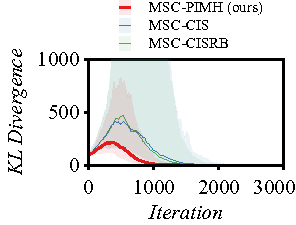
\includegraphics[scale=0.85]{figures/gaussian_01.pdf}
  }
  \subfloat[\(N=2^4\)]{
    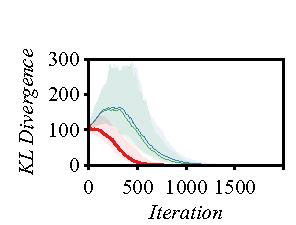
\includegraphics[scale=0.85]{figures/gaussian_02.pdf}
  }
  \subfloat[\(N=2^6\)]{
    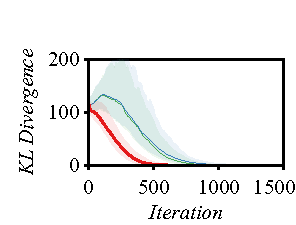
\includegraphics[scale=0.85]{figures/gaussian_03.pdf}
  }
  \caption{100-D isotropic Gaussian example with a varying computational budget \(N\).
    MSC-PIMH kernel converges faster than MSC-CIS with and MSC-CISRB regardless of \(N\).
    Also, the convergence of MSC-PIMH becomes more stable/monotonic as \(N\) increases.
    The solid lines are the median of 100 repetitions while the colored regions are the 80\% empirical percentiles.
  }\label{fig:gaussian}
  \vspace{-0.1in}
\end{figure*}

\section{Evaluations}\label{section:eval}
\subsection{Experimental Setup}
\paragraph{Implementation}
We implemented MSC with PIMH on top of the Turing~\citep{ge2018t} probabilistic programming framework.
Our implementation works with any model described in Turing, which automatically handles distributions with constrained support~\citep{JMLR:v18:16-107}.

\paragraph{Considered Baselines}
We compare MSC-PIMH against
\begin{enumerate*}[label=\textbf{(\roman*)}]
  \item  MSC using the CIS kernel (\textbf{MSC-CIS},~\citealt{NEURIPS2020_b2070693}), 
  \item  MSC using the CIS kernel with Rao-Blackwellization (\textbf{MSC-CISRB},~\citealt{NEURIPS2020_b2070693})
  \item the adaptive IS method using SNIS as introduced in Section~\ref{section:ivi_previous} (\textbf{SNIS}).
  \item the reweighted wake-sleep algorithm (\textbf{RWS},~\citealt{DBLP:journals/corr/BornscheinB14}),  
  \item and evidence lower-bound minimization (\textbf{ELBO},~\citealt{pmlr-v33-ranganath14}).
\end{enumerate*}
Specifically, we use automatic differentiation variational inference (ADVI,~\citealt{JMLR:v18:16-107}) implemented by Turing.

\begin{figure*}
  \centering
  \subfloat[Pima]{
    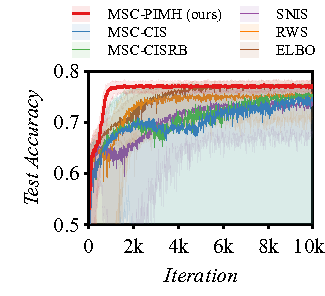
\includegraphics[scale=0.80]{figures/pima_02.pdf}
  }
  \subfloat[Heart]{
    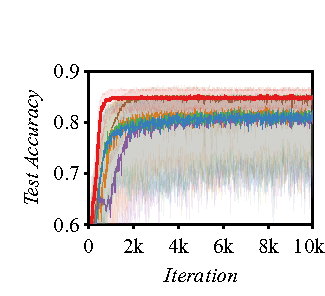
\includegraphics[scale=0.80]{figures/heart_02.pdf}
  }
  \subfloat[German]{
    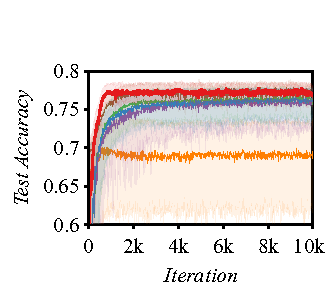
\includegraphics[scale=0.80]{figures/german_02.pdf}
  } \\
  \subfloat[Pima]{
    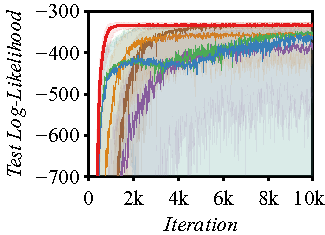
\includegraphics[scale=0.80]{figures/pima_03.pdf}
  }
  \subfloat[Heart]{
    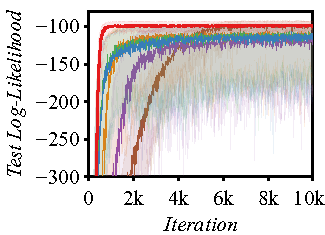
\includegraphics[scale=0.80]{figures/heart_03.pdf}
  }
  \subfloat[German]{
    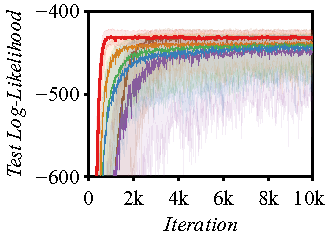
\includegraphics[scale=0.80]{figures/german_03.pdf}
  }
  \caption{Test accuracy and log-likelihood of logistic regression problems.
    The solid lines are the median of 100 repetitions while the colored regions are the 80\% empirical percentiles.
  }\label{fig:logistic}
\end{figure*}

\paragraph{Reinterpreting RWS}
The original RWS algorithm assumes that independent samples from \(p(\vz\mid\vx)\) are available possibly with an additional cost.
It uses these independent samples for estimating the gradient once every \(K\) steps, and uses SNIS for the rest.
In our setting, we do not assume that independent samples from \(p(\vz\mid\vx)\) are available.
Instead, we reinterpret the idea of RWS of alternating between expensive and cheap estimates, and alternate between SNIS estimates and HMC estimates.
HMC shows excellent statistical performance in practice, but is much expensive as it requires multiple gradients \(\nabla_{\vz} p(\vz, \vx)\) for generating only a single samples.
As originally recommended by~\citet{DBLP:journals/corr/BornscheinB14}, we set \(K=5\).

\subsection{Isotropic Gaussian}
We first perform experiments with a 100-D isotropic multivariate Gaussian distribution.
The KL divergence between two multivariate Gaussian is available in a closed form, enabling exact analysis.
We first compare the performance of MSC-PIMH, MSC-CIS, and MSC-CISRB with respect to the N (number of proposals for MSC-CIS(RB); number of parallel chains for MSC-PIMH).
The results are shown in Figure~\ref{fig:gaussian}.
While MSC-PIMH shows some level of overshoot wih \(N=4\), it shows monotonic convergence with larger \(N\).
On the other hand, both MSC-CIS and MSC-CISRB overshoots even with \(N=64\).
This clearly shows that our PIMH kernel enjoys better gradient estimates compared to the CIS kernel.

\subsection{Hierarchical Logistic Regression}
\paragraph{Experimental Setup}
We now evaluate MSC-PIMH on logistic regression problems.
We consider the Pima Indians diabetes (\textbf{pima}), German credit (\textbf{german}), and heart disease (\textbf{heart}) datasets.
10\% of the datapoints in each dataset were excluded from training and used as test data.
The train-test splits were chosen randomly in each of the 100 repetitions.

Instead of the common single-level porbit/logistic regression models used in VI, we choose a more complex hierarchical logistic regression model \\
\begin{equation}
y_i \sim \text{Bernoulli-Logit}\,(p),\;
p \sim \mathcal{N}(\vx_i^{\top}\symbf{\beta} + \alpha,\, \sigma_{\alpha}^2),\;
\symbf{\beta} \sim \mathcal{N}(\symbf{0},\, \sigma_{\beta}^2 \mI),\;
\sigma_{\beta},\,\sigma_{\alpha} \sim \mathcal{N}^{+}(0, 1.0)
\end{equation}
where \(\mathcal{N}^+(\mu, \sigma)\) is a positive constrained normal distribution with mean \(\mu\) and standard deviation \(\sigma\), \(\vx_i\) and \(y_i\) are the feature vector and target variable of the \(i\)th datapoint.
The extra degrees of freedom \(\sigma_{\beta}\) and \(\sigma_{\alpha}\) make this model relatively more challenging.

%
\begin{wrapfigure}{r}{0.4\textwidth}
  \vspace{-0.3in}
  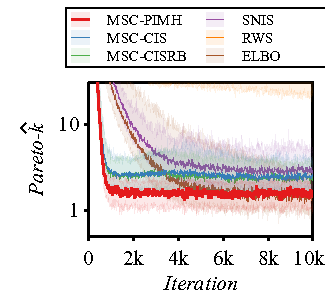
\includegraphics[scale=0.8]{figures/german_01.pdf}
  \caption{Pareto-\(\widehat{k}\) statistic.}\label{fig:paretok}
  \vspace{-0.1in}
\end{wrapfigure}
%
\paragraph{Results Summary}
The test accuracy and test log-likelihood results are shown in Figure~\ref{fig:logistic}.
MSC-PIMH was the fastest to converge on all of the datasets.
Despite being able to utilize high-quality samples generated from HMC, RWS failed to achieve similar level of performance to MSC-PIMH.
However, compared to MSC-CIS and MSC-CISRB, it converged faster.
Among the two, MSC-CISRB performed only marginally better than MSC-CIS.
Meanwhile, SNIS was the slowest to converge among inclusive VI methods.
Lastly, despite being much slower to converge, ELBO achieved similar level of performance to MSC-PIMH.

\paragraph{Inclusive VI v.s. Exclusive VI}
The test accuracy and log-likelihood results in Figure~\ref{fig:logistic} can convey a deceptive conclusion that inclusive and exclusive VI deliver similar results.
However, in the perspective of parameter inference, both choose very different optimization paths.
This is shown in Figure~\ref{fig:paretok} through the pareto-\(\widehat{k}\) diagnostic~\citep{vehtari_pareto_2021, NEURIPS2020_7cac11e2}, which determines how reliable are the importance weights computed using \(q_{\vlambda}\).
While the test accuracy suggests that ELBO converged around \(t=2000\), the pareto-\(\widehat{k}\) takes much longer to converge (about \(t=5000\)).
This shows that, even if their predictive performance is similar, the inclusive VI chooses a path that has better density coverage as expected.

\subsection{General Bayesian Inference}

\paragraph{Did inclusive VI live up to its hype?}
\citet{dhaka_challenges_2021} showed that, inclusive VI works against our intuitions in higher dimensions.
However, if the posterior is strongly correlated, inclusive VI can fail even in lower dimensions.
On the other hand, if the posterior is not strongly correlated, our experiments suggest that inclusive VI can work better than exclusive VI.
Furthermore, posterior correlation affects all methods relying on the mean-field approximation, not only inclusive VI.


%%% Local Variables:
%%% TeX-master: "master"
%%% End:
